\documentclass[conference]{IEEEtran}
\IEEEoverridecommandlockouts
% The preceding line is only needed to identify funding in the first footnote. If that is unneeded, please comment it out.
\usepackage{cite}
\usepackage{amsmath,amssymb,amsfonts}
\usepackage{algorithmic}
\usepackage{graphicx}
\usepackage{textcomp}
\usepackage{xcolor}
\usepackage{hyperref}
\usepackage{array}
\usepackage{caption} % for \captionsetup command
\usepackage{svg}






\newcommand{\gr}[1]{\textcolor{green}{#1}}

\def\BibTeX{{\rm B\kern-.05em{\sc i\kern-.025em b}\kern-.08em
    T\kern-.1667em\lower.7ex\hbox{E}\kern-.125emX}}
\begin{document}

\title{Mamba-Based Tumor Segmentation\\
    \thanks{$\dagger$ Equal contributions}
}

\author{\IEEEauthorblockN{Clay Crews$^{\dagger}$}
    \IEEEauthorblockA{\textit{Department of Computer Science} \\
        \textit{University of South Carolina}\\
        Columbia, SC, United States \\
        jccrews@email.sc.edu}
    \and
    \IEEEauthorblockN{Lexington Whalen$^{\dagger}$}
    \IEEEauthorblockA{\textit{Department of Computer Science} \\
        \textit{University of South Carolina}\\
        Columbia, SC, United States\\
        LAWHALEN@email.sc.edu}
}

\maketitle

\begin{abstract}
    U-net and transformer-based architectures have dominated medical image segmentation, particularly for tumor segmentation from brain MRI scans. However, recent advances in Structured State Space Sequence Models (SSMs) present a promising alternative with comparable modeling power to transformers but linear scalability in sequence length, making them well-suited for large medical images.

    We propose exploring the application of the Mamba block, a variant of SSMs, for tumor segmentation in brain MRI scans. By leveraging selective state spaces, Mamba blocks can potentially enhance the efficiency and effectiveness of tumor segmentation while maintaining linear scalability.

    Our methodology involves implementing and fine-tuning a Mamba-based architecture on a dataset of annotated brain MRI scans. We will evaluate the model's performance using standard segmentation metrics and compare the results with U-net and transformer-based approaches. We open-source the code here: \href{https://github.com/lxaw/mamba-tumor-seg}{https://github.com/lxaw/mamba-tumor-seg}.
\end{abstract}

\begin{IEEEkeywords}
    Mamba, Segmentation, Selective State Spaces
\end{IEEEkeywords}

\section{Introduction}
MRI imaging to identify brain tumors has naturally been a target for accurate image segmentation through the use of machine learning (ML) architecture. The use of computer-aided diagnosis of tumors can be crucial to quickly identify tumors and determine a course of action for the patient. Gliomas are the most common primary brain malignancy with varying degrees of aggressiveness in the brain. The protocol for MRI image annotation of these tumors consists of the following labels: the whole tumor extent, the tumor core, the non-enhancing/necrotic tumor region, and regions of low grade gliomas \cite{bakas2019identifying}. These annotations of an MRI are used to determine the size and severity of a tumor.

To accurately segment these images, picking out the small features of the image becomes the focus. The use of the U-Net architecture, presented by Ronneberger, Fischer, and Brox \cite{ronneberger2015unet}, has had success in MRI image segmentation. U-Net builds on the approach of fully convolutional networks by improving the limitation on the large amount of data needed to accurately train the model. Very few training images are needed due to the contracting and expansive paths in this architecture. In the contracting path, images are downsampled and pooled along with increasing the number of feature channels. Each downsampled resolution produces a multi-channel feature map. The expansive path up samples and combines with each segmentation feature map from the contracting layer to localize features in the image. A 1x1 convolution layer is applied to the final image to map the large feature vector to a selected number of classes. All of this essentially creates a feature map where each pixel’s relevance is taken into account and evaluated in the end result. An approach using the U-Net architecture would provide the detailed analysis needed for tumor annotation.

An arising issue in the complex recurrent or convolutional neural networks used for image segmentation is the length of the sequences given as input. Maintaining relevance of the current area of an image in relation to the rest of the image is key for more accurate segmentation. An approach with the Transformer architecture has a large emphasis on learning specific features in an image, outlined by Vaswani et al. 2017 \cite{vaswani2023attention}. This architecture follows an encoder-decoder pattern, connected through an attention mechanism, a transformer block. Transformer blocks show capability of learning long-distance dependency throughout an input image. In the self-attention mechanism for this block, a single element in a given sequence is compared to all of the elements in the sequence. However, this mechanism becomes computationally very expensive when it comes to long sequences.

Selective State Spaces (SSMs) pose an improvement in computational efficiency over Transformers for this long dependency range. SSMs represent the relevance and context of different parts of the input sequence giving selective attention. This model is widely used in control theory for time variant systems and in fields such as computational neuroscience. Selective attention is very efficient in handling long sequences over time and presents a more localized context of the data. Sections of sequences that deserve attention are represented by the model and will dynamically update these values to reflect the contextual relevance.

Making use of Structured State Spaces, presented by Gu, Goel, and Ré \cite{gu2022efficiently}, for their superiority in long range dependency tasks, a specific type of SSM, the Mamba architecture, by Gu and Dao \cite{gu2023mamba}, proposed a foundational model to operate on arbitrary sequences from a variety of inputs in the domain of sequence modeling. This model achieves the power of Transformers while scaling linearly in sequencing length to be computationally efficient. Additionally, the selection mechanism of Mamba improves on an SSMs ability to focus on or ignore sections in an input sequence by parameterizing the parameters of an SSM to reflect the current context of the input. The Mamba model and its application to brain tumor MRI imaging segmentation will be evaluated in this project.


\section{Mamba}
Mamba \cite{gu2023mamba} is a recently proposed architecture that combines the modeling power of Transformers with the linear scaling efficiency of state space models (SSMs). The key idea is to augment SSMs with a selection mechanism that allows the model parameters to vary based on the input, enabling it to perform content-aware reasoning.
Standard SSMs map an input sequence $x(t)$ to an output $y(t)$ via a latent state $h(t)$ using a linear time-invariant system:
\begin{align*}
    h'(t) & = \mathbf{A}h(t) + \mathbf{B}x(t) \\
    y(t)  & = \mathbf{C}h(t) + \mathbf{D}x(t)
\end{align*}

where the parameter matrices $\mathbf{A}$, $\mathbf{B}$, $\mathbf{C}$, $\mathbf{D}$ are fixed. In the original paper, the $\mathbf{D}$ matrix is considered only as a skip connection, and thus as it does not directly play a role in the differential equation, was ignored. This allows SSMs to be computed efficiently as a convolution. However, the time-invariance means the model cannot change its behavior for specific inputs, making it difficult to solve tasks requiring selective focus, such as selective copying or induction heads \cite{gu2023mamba}.
Mamba introduces a selection mechanism where the SSM parameters $\mathbf{B}$, $\mathbf{C}$, $\Delta$ (the state step size) vary for each input token $x_t$. This allows the model to selectively propagate or forget information based on the current token. The selective SSM is computed using a parallel scan operation to maintain linear complexity.
The Mamba block interleaves the selective SSM with linear projections, convolutions, and activations:
\begin{enumerate}
    \item Linear projection to expand the embedding dimension
    \item Convolution to mix information between dimensions
    \item Selective SSM via parallel scan to efficiently propagate information
    \item Linear projection to get back to the target embedding size
\end{enumerate}
These blocks are stacked to form the Mamba architecture. Compared to Transformers, Mamba can achieve comparable modeling performance while scaling linearly in sequence length rather than quadratically \cite{gu2023mamba}. Overall, the selective SSM leverages the strengths of RNNs, CNNs and Transformers - it maintains an unbounded context window like RNNs, can be parallelized like CNNs, and achieves content-aware reasoning like Transformers, while being more efficient than all three. This makes Mamba a promising foundation model for processing long sequences across various domains.



\section{Related Works}
Prior to an analysis of how the Pyramidal U-Mamba compares, we shall explain what models we chose for comparison and why.

For this our analysis, we compare four models against our own developed ones. The models are U-Net\cite{ronneberger2015unet}, ResNet18 \cite{he2015deep}, ResNet50, U-Mamba\cite{ma2024umamba}, and SegViT\cite{dosovitskiy2021image}. Below we explain our choices.
\subsection{U-Net}
The core idea behind U-Net is to complement a traditional contracting network with successive layers that replace pooling operations with upsampling operators. These upsampling layers aim to increase the resolution of the output. Subsequent convolutional layers can then learn to assemble a precise output based on this high-resolution information \cite{ronneberger2015unet}.
A key modification in the U-Net architecture is the inclusion of a large number of feature channels in the upsampling part. This allows the network to effectively propagate contextual information to higher resolution layers. As a result, the expansive path of the network becomes more or less symmetric to the contracting part, leading to a distinctive U-shaped architecture. To predict pixels at the border regions of the image, the missing context is extrapolated by mirroring the input image. This tiling strategy is crucial for applying the network to large images, as it circumvents resolution limitations imposed by GPU memory constraints \cite{ronneberger2015unet}. Due to its encoder-decoder architecture, skip connections, multi-scale feature extraction, and its efficiency, U-Net has been used in many denoising and diffusion models. For instance, DDPMs (Denoising Diffusion Probabilistic Models) use an architecture similar to U-Net for denoising and sample generation \cite{ho2020denoising} while the popular Stable Diffusion architecture uses a U-Net based architecture for the diffusion process \cite{rombach2021highresolution}. We have chosen to compare our novel segmentation architecture against the U-Net architecture due to its well-established reputation and widespread adoption in the field of medical image segmentation.

\subsection{ResNet}
We have also selected ResNet18 and ResNet50 as additional benchmarks. These architectures, introduced by He et al. in their seminal work "Deep Residual Learning for Image Recognition" \cite{he2015deep}, have revolutionized the field of deep learning by addressing the problem of vanishing gradients in deep neural networks. The key innovation in ResNets is the introduction of residual connections, which allow the network to learn residual functions with reference to the input layer, thereby facilitating the training of much deeper networks. ResNet18 and ResNet50, with 18 and 50 layers respectively, have been widely adopted in various computer vision tasks, including image classification, object detection, and segmentation. These models have demonstrated exceptional performance and generalization ability across diverse datasets. By comparing our proposed architecture against ResNet18 and ResNet50, we aim to assess its effectiveness in relation to these well-established and highly influential architectures. This comparison will provide valuable insights into the capabilities of our model and its potential to advance the state-of-the-art in image segmentation tasks.
\subsection{U-Mamba}
As our model takes much inspiration from the recently developed U-Mamba design \cite{ma2024umamba}, we also choose to incorporate it in our comparison. U-Mamba addresses these limitations by introducing a novel hybrid CNN-SSM block that leverages the strengths of both architectures. The convolutional layers in the block are responsible for local feature extraction, while the State Space Sequence Models (SSMs) \cite{gu2022efficiently}, a new family of deep sequence models, are known for their strong capability in handling long sequences and capturing long-range dependencies. By integrating these two components, U-Mamba achieves a balance between local and global information processing, enabling it to effectively handle long-range dependencies in biomedical image segmentation tasks. Moreover, U-Mamba incorporates a self-configuring mechanism that allows it to automatically adapt to various datasets without manual intervention, enhancing its versatility and usability.
\subsection{SegFormer}
SegFormer \cite{xie2021segformer} is a transformer-based semantic segmentation model that employs a hierarchical structure and a novel attention mechanism called Efficient Self-Attention (ESA). The SegFormer architecture consists of a transformer encoder for capturing long-range dependencies and a lightweight All-MLP decoder for generating high-resolution segmentation masks. The ESA module reduces the computational complexity of self-attention by performing attention operations in a local window and aggregating global information through a depth-wise convolution. This allows SegFormer to efficiently process high-resolution images while capturing both local and global context. Moreover, SegFormer introduces a position-sensitive embedding scheme that encodes both spatial and channel-wise information, enhancing the model's ability to capture fine-grained details. By comparing U-Mamba against SegFormer, we aim to evaluate the effectiveness of our hybrid CNN-SSM approach in relation to the transformer-based segmentation mechanism employed by SegFormer. This comparison will provide insights into the strengths and weaknesses of both architectures and their ability to handle complex biomedical image segmentation tasks. Furthermore, it will help us understand the potential of transformer-based approaches and hybrid approaches in advancing the state-of-the-art in biomedical image segmentation.

\subsection{UltraLight VM-UNet}
The UltraLight VM-UNet \cite{wu2024ultralight} is a lightweight neural network architecture designed for skin lesion segmentation tasks. It is built upon the Vision Mamba module, which is a state-space model (SSM) that can efficiently handle long-range dependencies in sequences, making it well-suited for image segmentation tasks.

The key innovation of the UltraLight VM-UNet is the proposed Parallel Vision Mamba Layer (PVM Layer), which processes deep features in parallel using multiple Vision Mamba blocks. Specifically, the input feature map is split into multiple sub-feature maps, each processed by a separate Vision Mamba block with a reduced channel count. This parallel processing approach allows the UltraLight VM-UNet to maintain high segmentation performance while significantly reducing the number of parameters and computational complexity.

The UltraLight VM-UNet is reported to have only 0.049 million parameters and a computational cost of 0.060 GFLOPs, which is significantly lower than traditional convolutional neural networks and transformers used for image segmentation tasks. Despite its lightweight nature, the authors demonstrate that the UltraLight VM-UNet achieves competitive performance on three publicly available skin lesion segmentation datasets, outperforming several state-of-the-art lightweight models.

The success of the UltraLight VM-UNet can be attributed to the authors' in-depth analysis of the key factors influencing the parameters of the Vision Mamba module. By identifying the number of input channels as a critical factor affecting the parameter count, they were able to design the PVM Layer to process features in parallel while keeping the overall channel count constant, leading to a significant reduction in parameters without compromising performance.

\section{Proposed Methodology}
In this paper, we strive to maintain high accuracy in our image segmentation while also keeping low parameter counts. We primarily seek to use pyramidal pooling modules \cite{zhao2017pyramid} to improve accuracy, and use a variant of the Mamba \cite{gu2023mamba} architecture inspired by \cite{wu2024ultralight} to maintain small parameter sizes.

\section{Input Data}\label{sec2}
We shall be using a Brain MRI segmentation dataset found in \cite{dataset}. This dataset has been used in several papers regarding classification of the shape and severity of tumors, and provides an adequate dataset for research purposes in the field of medical image analysis, particularly in the area of brain MRI segmentation. Researchers have utilized this dataset in various studies focusing on the classification of tumor shapes and the assessment of tumor severity. With its comprehensive collection of brain MRI scans, along with corresponding segmentation masks, the dataset offers valuable resources for developing and evaluating algorithms aimed at automating tumor detection and analysis.

The dataset contains brain MRI images along with their segmentation masks for 110 patients. There were a total of 3143 train images, 393 validation images, and 393 test images. The distribution of the tumor and non-tumor images is shown in Figure \ref{fig:datastats}.


\section{Output Data}\label{sec3}
The output of this model shall be segmentation masks for new, never before seen images.
\begin{figure}[!t]
    \centering
    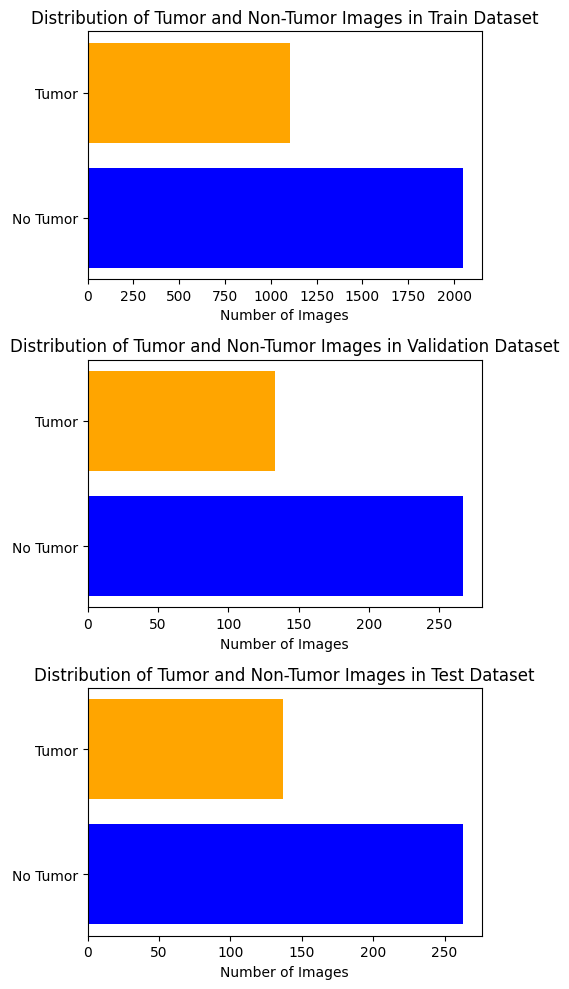
\includegraphics[width=\columnwidth]{imgs/data_stats.png}
    \caption{Distributions of tumor and non-tumor images in the train, validation, and test datasets.}
    \label{fig:datastats}
\end{figure}


\section{Our Models}

Inspired by \cite{ma2024umamba} and \cite{wu2024ultralight}, we sought to implement both models on a different problem: tumor segmentation.

Our goal was to 1) maintain dice scores comparable to state-of-the-art (SOTA) methods such as those listed above, while 2) being smaller than those above.

We now go into what we did for each of our models.


\subsection{UMambaBot-PP}

This model incorporates pyramidal pooling, which is a strategy used in convolutional neural networks (CNNs) to capture context and incorporate multi-scale information \cite{zhao2017pyramid}. Pyramidal pooling involves parallel pooling operations at different scales, followed by concatenation of the resulting feature maps. This approach has been shown to improve the performance of CNNs in various computer vision tasks, including segmentation, by enabling the model to capture both local and global context.

In our UMambaBot-PP model, we integrated pyramidal pooling into the U-Mamba architecture, aiming to leverage the strengths of both the Mamba module and multi-scale feature extraction.

% Unsure why this comment line is giving me troubles !!

\subsection{UL-VM-UNet-v1}
For UL-VM-UNet-v1, the initial channel list was modified from [8, 16, 24, 32, 48, 64] to [16, 32, 64, 128, 256], increasing the number of channels at each step of the encoder and decoder. Additionally, the depth of the U-Net was reduced by one layer to keep the parameter count low while increasing the number of parameters in each step. The intention was to improve performance by increasing the capacity of the model while maintaining a reasonable parameter count.

\subsection{UL-VM-UNet-v2}
In UL-VM-UNet-v2, the number of parallel branches in the Parallel Vision Mamba (PVM) block was increased from 4 to 8. This modification directly decreases the parameter count, further proving the idea proposed in the UltraLight VM-UNet paper \cite{wu2024ultralight} that processing features in parallel with reduced channel counts can significantly reduce parameters while maintaining performance.

\subsection{UL-VM-UNet-v3}
UL-VM-UNet-v3 combines the modifications from UL-VM-UNet-v1 and UL-VM-UNet-v2. It increases the number of parallel branches in the PVM block to 8 and modifies the channel list to [16, 32, 64, 128, 256]. Additionally, the depth of the U-Net was reduced to 5 layers. This approach aims to balance the trade-off between model capacity and parameter efficiency.

\subsection{UL-VM-UNet-v4}
This model incorporates pyramidal pooling, similar to UMambaBot-PP, but within every PVM block in both the encoder and decoder in the UltraLight VM-UNet architecture. The goal was to leverage the benefits of multi-scale feature extraction while maintaining the parameter efficiency of the UltraLight VM-UNet.

\subsection{UL-VM-UNet-v5}
UL-VM-UNet-v5 is meant to be a comparison to the -v4 and -v6 UltraLight variations. This model trained and performed well with 1.1M parameters. Incorporating pyramidal pooling on the UL network scored slightly worse than without pyramidal pooling but required approximately 400,000 more parameters. 

\subsection{UL-VM-UNet-v6}
Another variation to further test the effects of incorporating pyramidal pooling in the UltraLight VM-UNet architecture was made by only using pyramidal pooling in the bottleneck layer, similarly done in UMambaBot-PP. The main goal here, again, was to integrate pyramidal pooling for the benefit of multi-scale feature extraction while keeping a low parameter count.


\section{Results}
We now compare our models against ResNet18, ResNet50, standard U-Mamba bottleneck, UNet, and UltraLight VM-UNet. We train for 100 epochs on all models, and use dice-loss with Adam optimizer. We train on roughly 3000 images, and validate on roughly 400. we then test on roughly 400. We show the distributions of our data in Figure \ref{fig:datastats}.
Model results are shown in Table \ref{tab:model_comparison} and Figures \ref{fig:balls},\ref{fig:segs}, with additional segmentation results in Appendix \ref{supp_figs}. Additional training information can be found in Appendix \ref{trainingpipeline}.


% Adjust the vertical spacing between rows
\renewcommand{\arraystretch}{1.25}
\begin{table}[ht]
    \centering
    \captionsetup{skip=6pt}
    \begin{tabular}{|l|c|c|}
        \hline
        \textbf{Model Name} & \textbf{\#Params (M) $\downarrow$} & \textbf{Dice Score $\uparrow$} \\
        \hline
        UMambaBot-PP(Ours) & 10.0 & 0.8867 \\
        UMambaBot & \textbf{9.8} & 0.8799 \\
        ResNet18 & 13.9 & 0.8648 \\
        ResNet50 & 42.9 & 0.8672 \\
        SegFormer & 17.8 & 0.8454 \\
        UNet & 7.8 & \textbf{0.8929} \\
        \hline\hline
        UL-VM-UNet & 0.049 & 0.79955 \\
        UL-VM-UNet-v1(Ours) & 0.20 & 0.8409 \\
        UL-VM-UNet-v2(Ours) & \textbf{0.042} & 0.8243 \\
        UL-VM-UNet-v3(Ours) & 0.176 & 0.8109 \\
        UL-VM-UNet-v4(Ours) & 1.1 & 0.8548 \\
        UL-VM-UNet-v5(Ours) & 0.7 & \textbf{0.8633} \\
        UL-VM-UNet-v6(Ours) & 0.77 & 0.8628 \\
        \hline
    \end{tabular}
    \caption{Comparison of different segmentation models.}
    \label{tab:model_comparison}
\end{table}

\begin{figure}[ht]
    \centering
    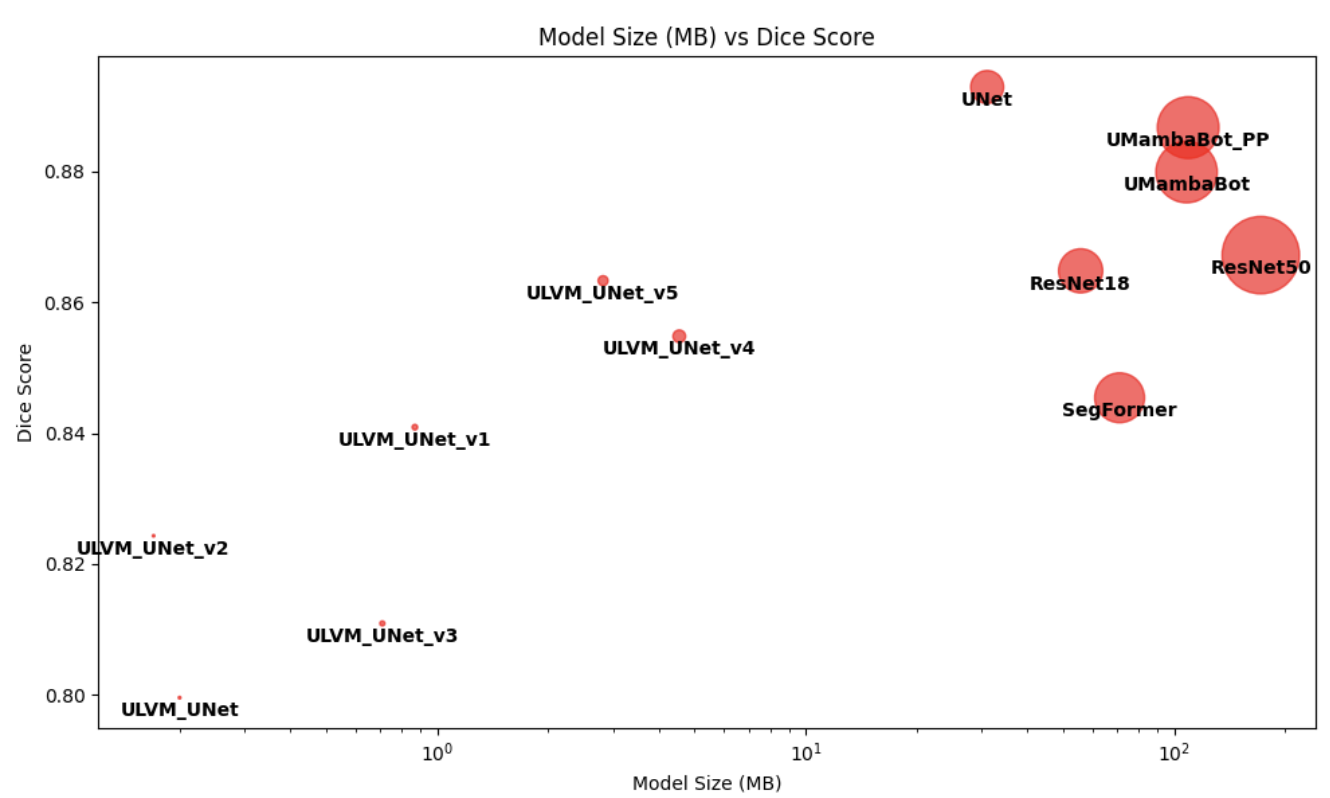
\includegraphics[width=\columnwidth]{imgs/balls.png}
    \caption{A scatter plot of Dice Score vs model parameter count, where "M" means "millions. The points are scaled to help represent size.}
    \label{fig:balls}
\end{figure}

\begin{figure}[ht]
    \centering
    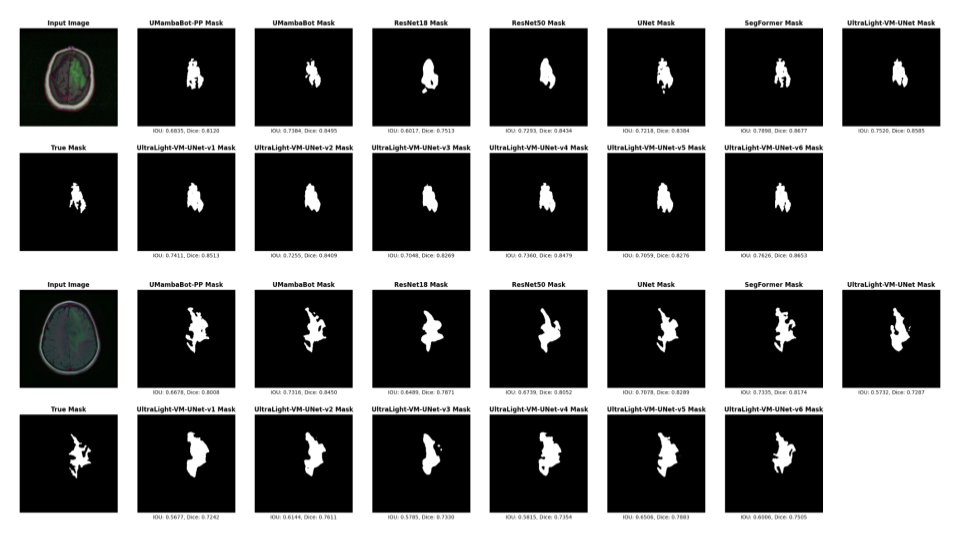
\includegraphics[width=\columnwidth]{imgs/tumor_seg_ex.png}
    \caption{Sample of segmentation results from each model and their dice score for the segmentation. (Additional samples in Appendix \ref{supp_figs})}
    \label{fig:segs}
\end{figure}

The integrated pyramidal pooling module to UMambaBot resulted in a slight increase in performance over the base model. However, UMambaBot-PP had an increase in parameter count by approximately 200,000 parameters. Additionally, our UL-VM-UNet-v2 achieved the lowest parameter count of 0.042 M with an increase over the original UltraLight VM-UNet architecture. Integrating a pyramidal pooling module to the UltraLight model, as done in UL-VM-UNet-v4 and -v6, resulted in an increase in parameter count with no change or a decrease in performance. 


\section{Conclusion}

In this work, we explored the application of Structured State Space Sequence Models (SSMs), particularly the Mamba architecture, for tumor segmentation from brain MRI scans. The Mamba architecture leverages selective state spaces, enabling efficient and effective segmentation while maintaining linear scalability.

Our experiments and comparisons with state-of-the-art (SOTA) models demonstrate the potential of the Mamba-based approach in both model size and segmentation accuracy. The smallest model, ULVM-Net-v2, achieved a compelling dice score of 0.8243 with only 0.042M parameters, achieving comparable performance to the larger ResNet50 model (42.9M params) with a dice score of 0.8672, while also outperforming the original UltraLight VM-UNet in terms of both parameter count and dice score.

While the traditional U-Net model achieved the highest dice score of 0.8929, our UMambaBot-PP model closely followed with a dice score of 0.8867. Notably, our Mamba-based UMambaBot-PP and UMambaBot models outperformed the Segformer transformer model, indicating the potential of Mamba-based approaches to surpass transformer-based models for this task.

We were able to make the UltraLight model smaller and more accurate on our task, further proving the potential of Mamba-based systems that prioritize compactness and efficiency. The selective state spaces and parallel processing strategies employed in our models enabled us to strike a balance between model size and segmentation accuracy.

Overall, this work contributes to the exploration of Structured State Space Sequence Models for medical image segmentation tasks. The Mamba architecture's ability to capture long-range dependencies while maintaining linear scalability positions it as a promising alternative to traditional convolutional and transformer-based approaches, especially in resource-constrained environments.

Future work could involve further refinements and optimizations of the Mamba-based models, as well as their application to other medical imaging modalities and segmentation tasks. Additionally, investigating the interpretability and robustness of these models could provide valuable insights for their deployment in real-world clinical settings.



\bibliographystyle{ieeetr}
\bibliography{refs}



\appendix
% Redefine the section numbering for the appendix (optional)
\renewcommand{\thesection}{\Alph{section}}
% First appendix section
\subsection{Training Pipeline} \label{trainingpipeline}
The training pipeline for our model consists of the following steps:

1. Data preprocessing: The dataset is split into training, validation, and test sets. The images are resized to a uniform size and normalized.

2. Model architecture: We employ a convolutional neural network (CNN) with the following layers: [Describe the layers and their configurations].

3. Training: The model is trained using the training set for 100 epochs with a batch size of 32. We use the Adam optimizer with a learning rate of 0.0003.

4. Evaluation: The trained model is evaluated on the validation set to monitor its performance and prevent overfitting. We use the dice loss metric.

5. Testing: Once the model achieves satisfactory performance on the validation set, it is tested on the held-out test set to assess its generalization ability.

% Second appendix section
\subsection{Supplementary Figures} \label{supp_figs}

\begin{figure*}[!h]
    \centering
    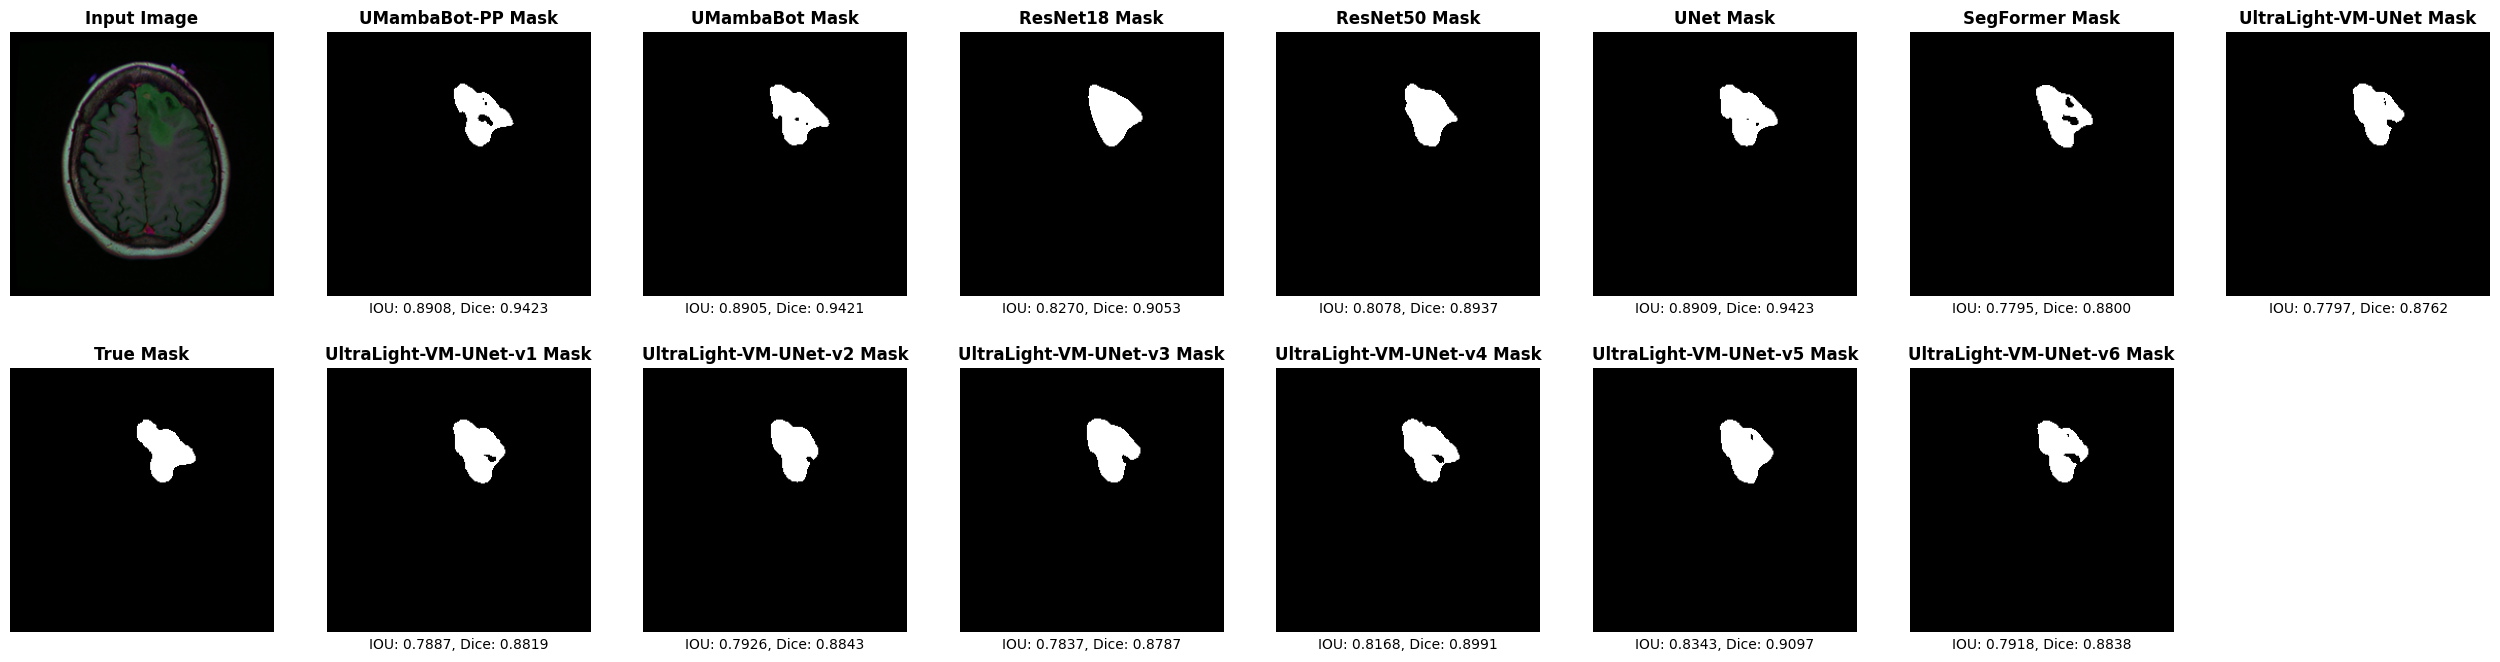
\includegraphics[width=\textwidth]{imgs/14_9.png}
\end{figure*}

\begin{figure*}[!h]
    \centering
    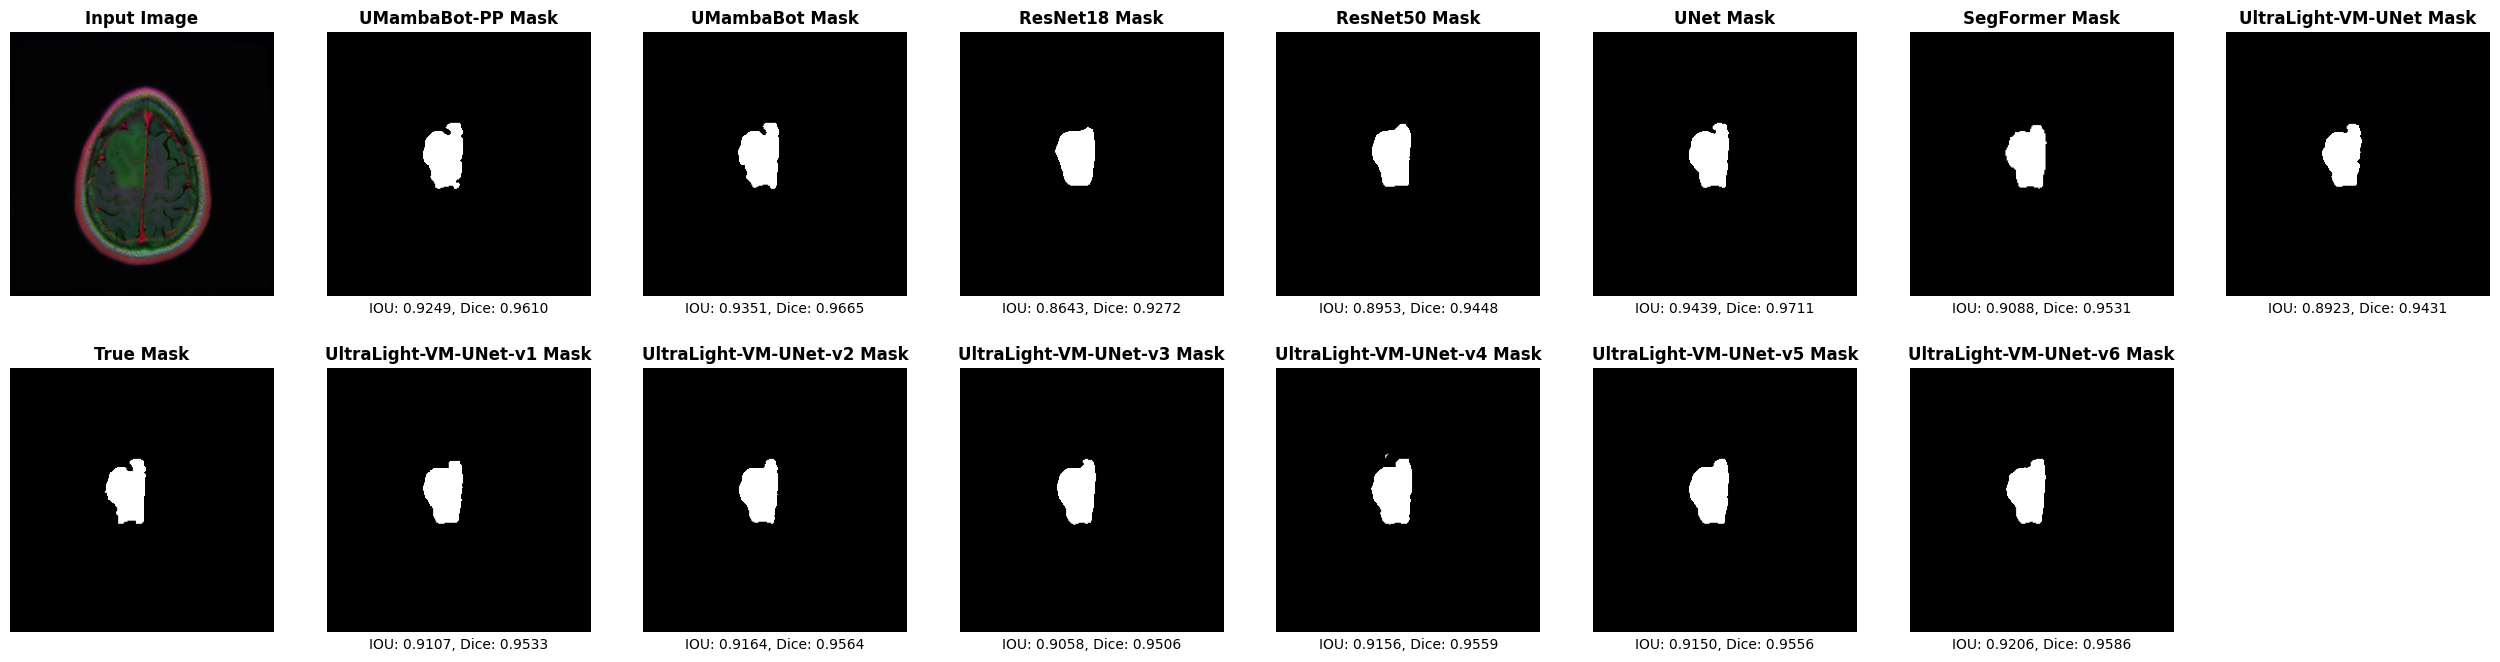
\includegraphics[width=\textwidth]{imgs/22_4.png}
\end{figure*}

\begin{figure*}[!h]
    \centering
    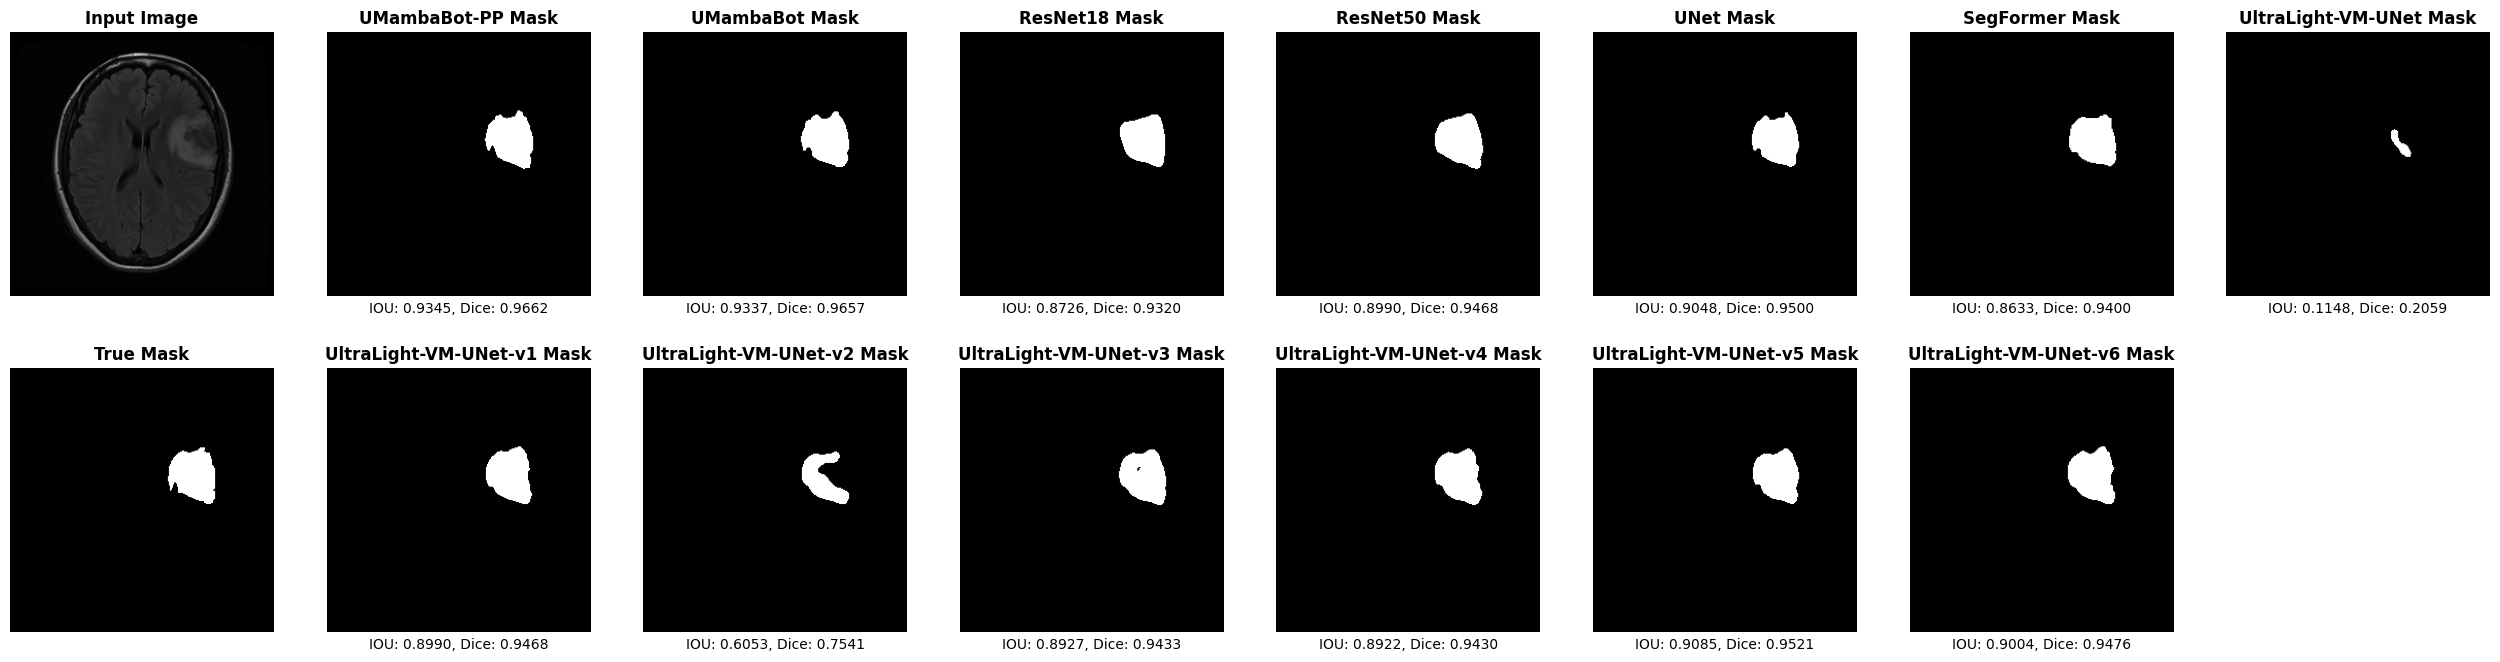
\includegraphics[width=\textwidth]{imgs/13_4.png}
    \caption{In some cases, such as this one, it was observed that models with too few parameters (UltraLight-VM-UNet, UltraLight-VM-UNet-v2) don't detect sections of the tumor during segmentation.}
\end{figure*}

\begin{figure*}[!h]
    \centering
    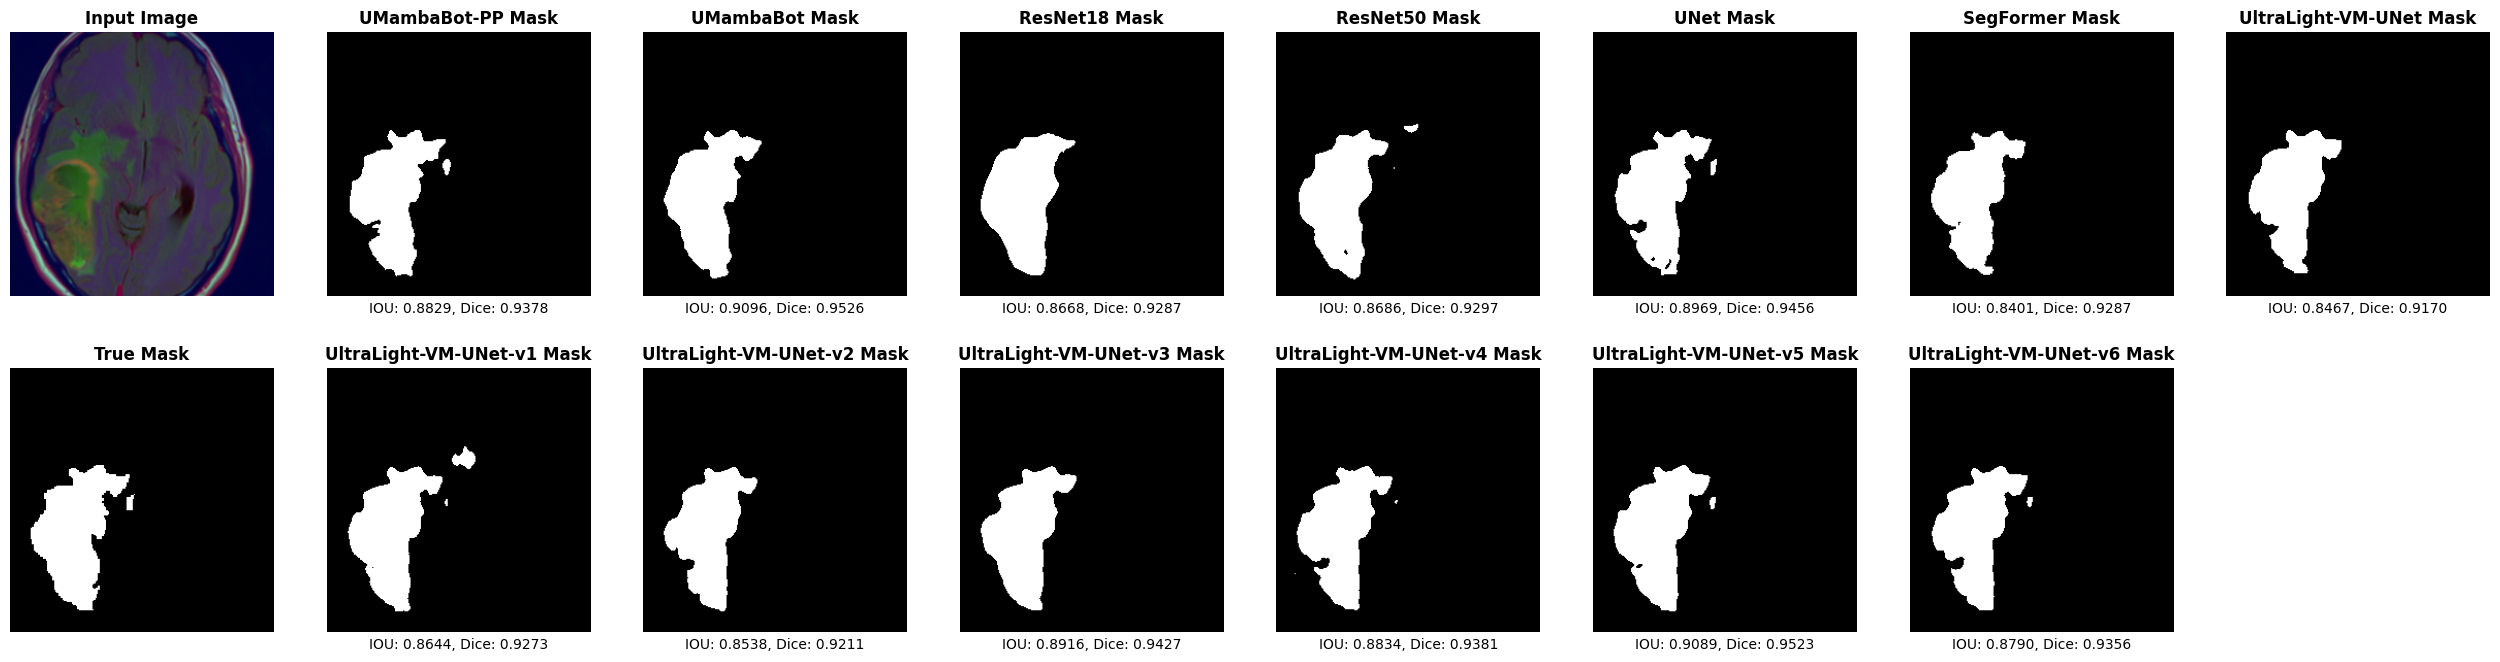
\includegraphics[width=\textwidth]{imgs/19_4.png}
    \caption{UltraLight-VM-UNet-v5 achieved segmentation results equivalent to UMambaBot with approximately 9.1 M less parameters.}
\end{figure*}

\begin{figure*}[!h]
    \centering
    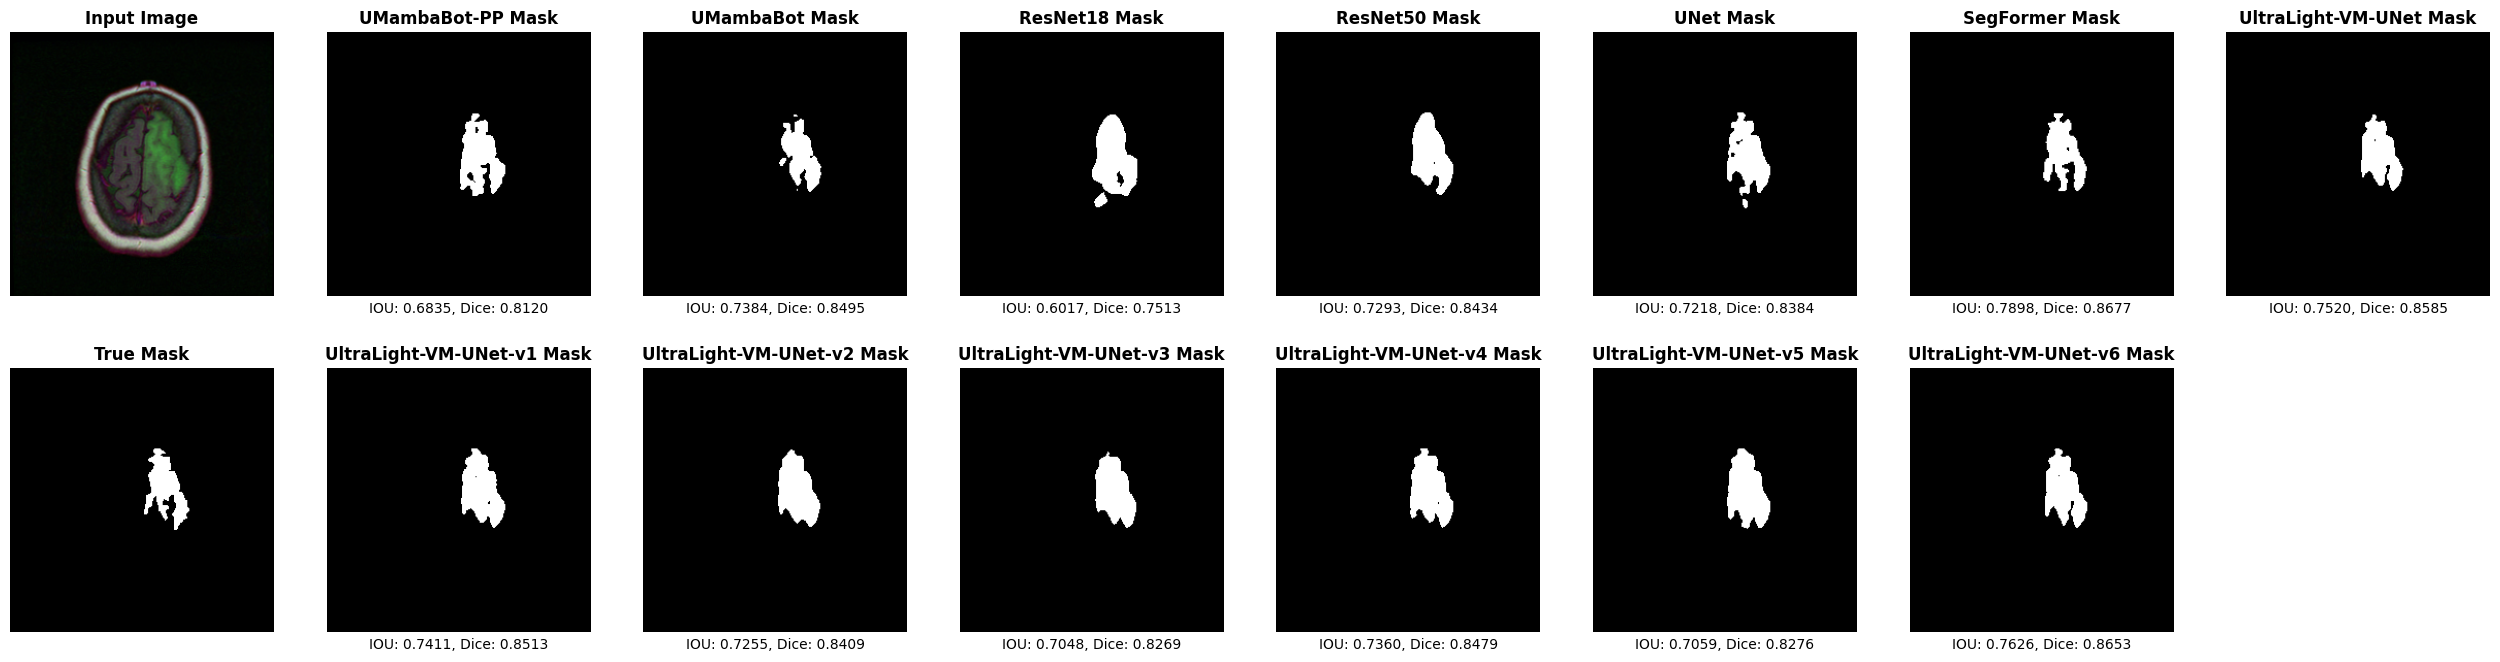
\includegraphics[width=\textwidth]{imgs/0_0.png}
    \caption{An example of models with pyramidal pooling in the PVM blocks (UltraLight-VM-UNet-v4, UltraLight-VM-UNet-v6) achieved an improvement over a model without (UltraLight-VM-UNet-v5).}
\end{figure*}

\begin{figure*}[!h]
    \centering
    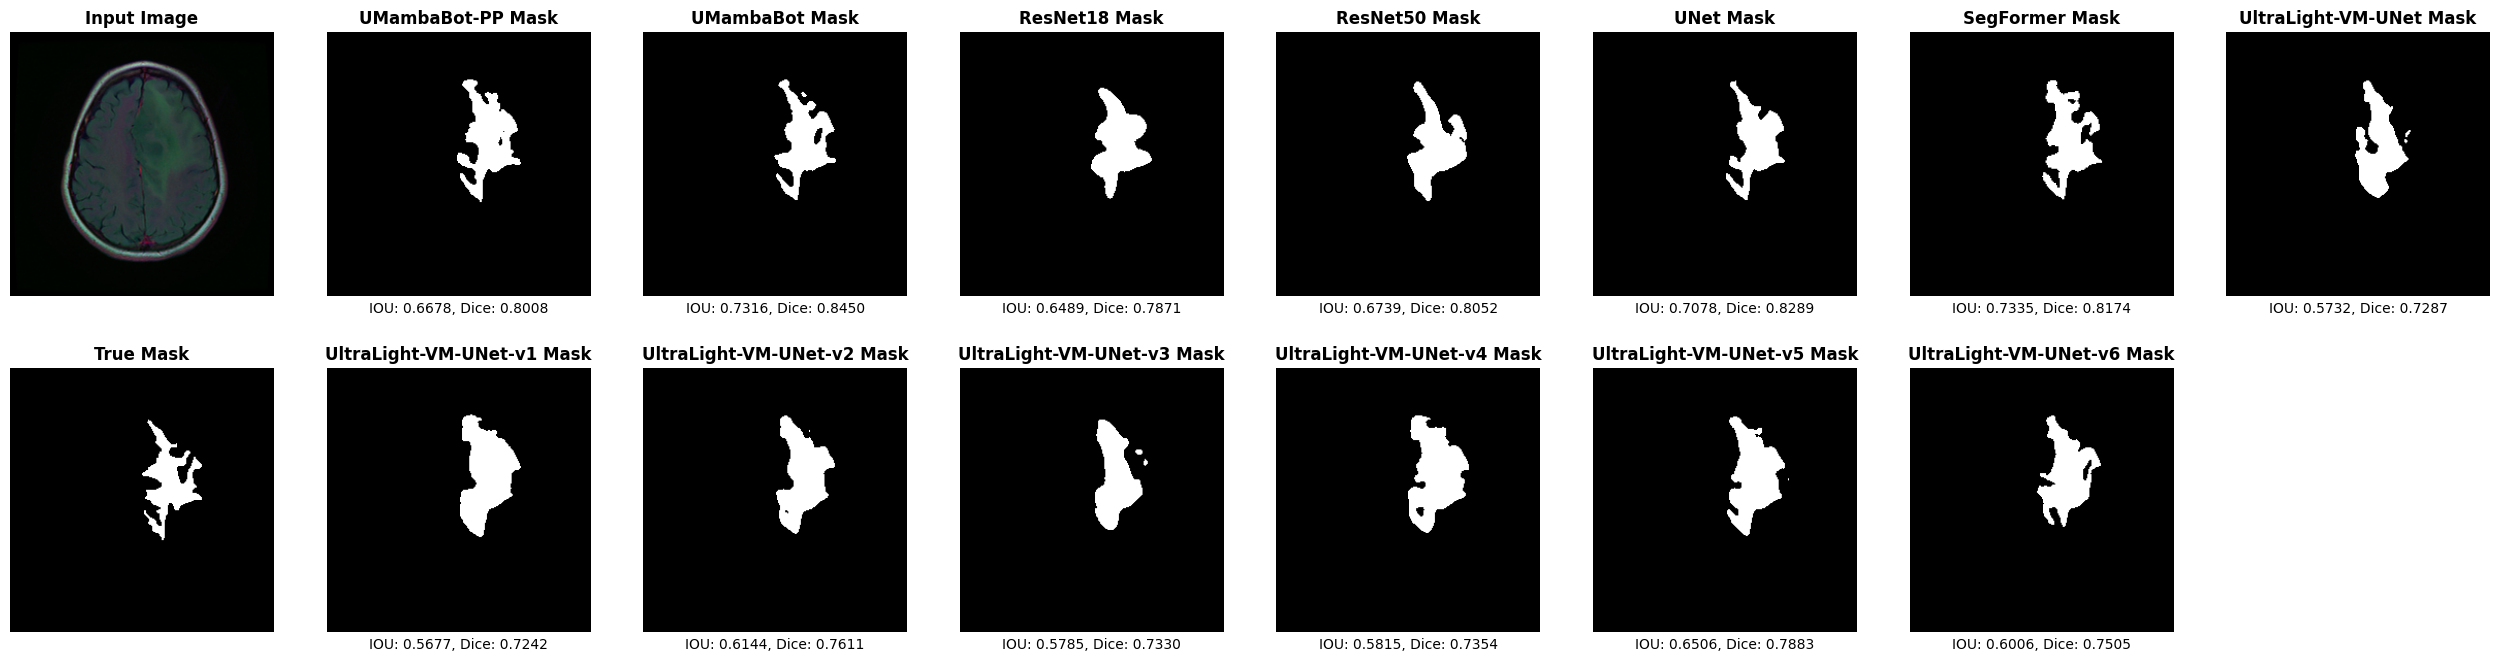
\includegraphics[width=\textwidth]{imgs/12_2.png}
\end{figure*}
\begin{figure*}[!h]
    \centering
    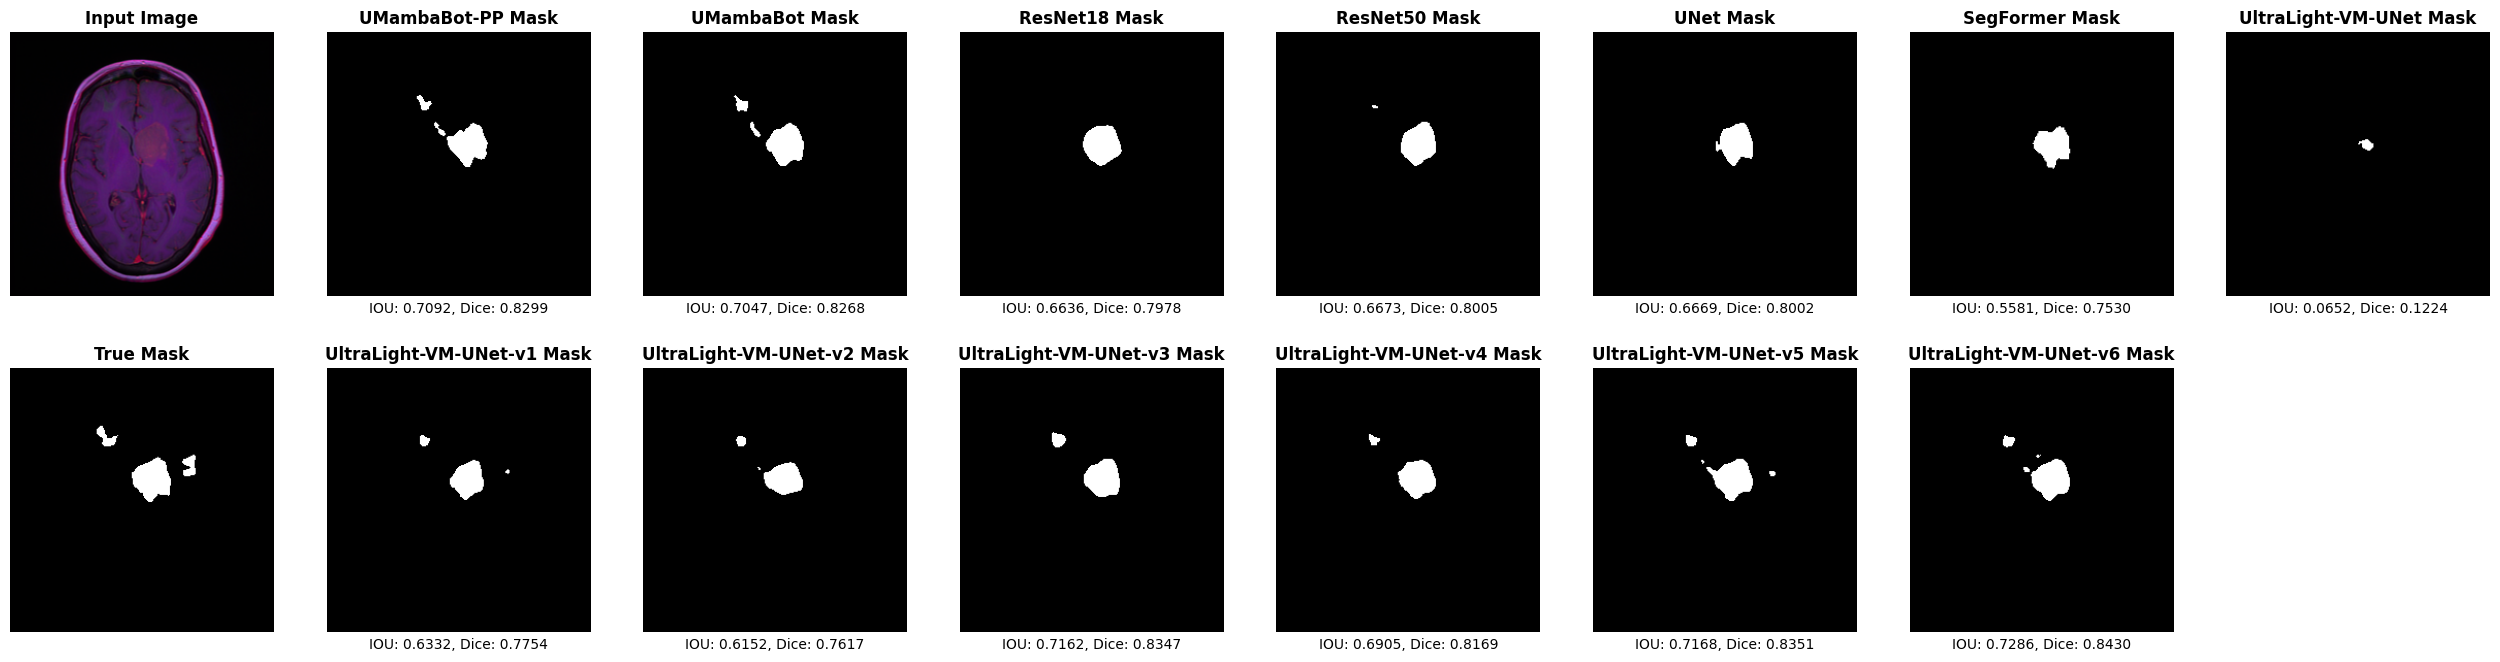
\includegraphics[width=\textwidth]{imgs/22_3.png}
\end{figure*}
\begin{figure*}[!h]
    \centering
    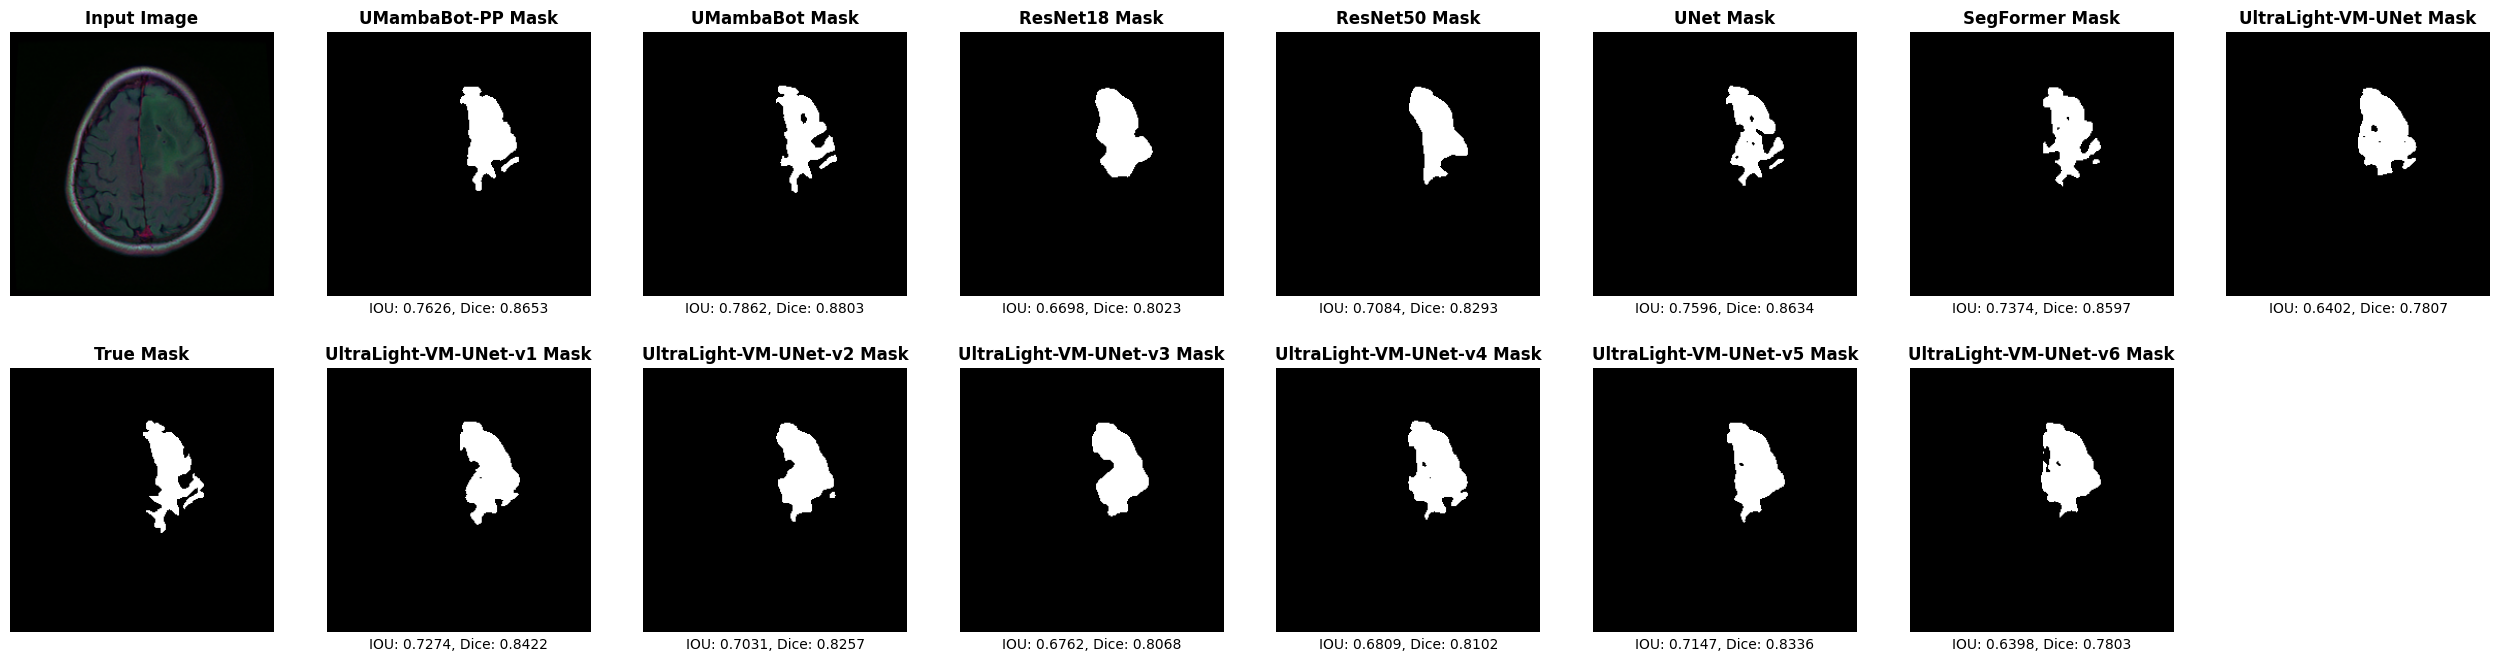
\includegraphics[width=\textwidth]{imgs/22_7.png}
\end{figure*}



\end{document}
